\documentclass[11pt]{article}
\usepackage[margin=0.85in]{geometry}
\usepackage{graphicx}
\usepackage{booktabs}
\usepackage{longtable}
\usepackage{float}
\usepackage{placeins}
\usepackage{amsmath}
\usepackage[hidelinks]{hyperref}
\title{D09-S Kgross GPIM Service-Life Sensitivity Analysis}
\author{Capacity Utilization US-Chile Source-of-Truth Pipeline}
\date{2026-07-01}
\begin{document}
\maketitle\tableofcontents\clearpage
\section{Purpose and Scope}
D09-S answers one validation question: whether the D06/D07 gross GPIM paths for ME and NRC are robust enough to proceed toward transformation planning after the D09-R report repair. The pass is human-facing and report-only.
The result is a sensitivity appendix, not a baseline replacement. All sensitivity stocks, ratios, and indices are REPORT\_ONLY, SENSITIVITY\_ONLY, NOT\_SOURCE\_OF\_TRUTH, NOT\_D06\_BASELINE, NOT\_MODEL\_READY, and require D10 or later authorization for transformation use.
\section{Locked Baseline and Report-Only Boundary}
The D06 baseline remains ME L=14 alpha=1.7 and NRC L=30 alpha=1.6. D09-S reads D06 guarded real investment and pKN paths, writes separate report outputs, and leaves D06/D07/D08/D09/D09-R artifacts unchanged.
\section{Nomura Literature Review: Discard, Survival, and Service Lives}
Nomura 2005 is not a U.S. service-life calibration source. It is a methodological and empirical warning source: service lives are asset-specific, discard data are noisy, single-period discard surveys can be biased, and office-building survival estimates depend on weighting and vintage adjustment. The extracted office-building values are S0 about 15.4 years, Sv about 22.2 years, and adjusted Sv-hat about 23.0 years.
Nomura-Futakami 2005 supports the principles of internal consistency, empirical verification, and reproducibility. D09-S operationalizes those principles by making service-life sensitivity visible without changing the locked baseline.
\begin{figure}[H]\centering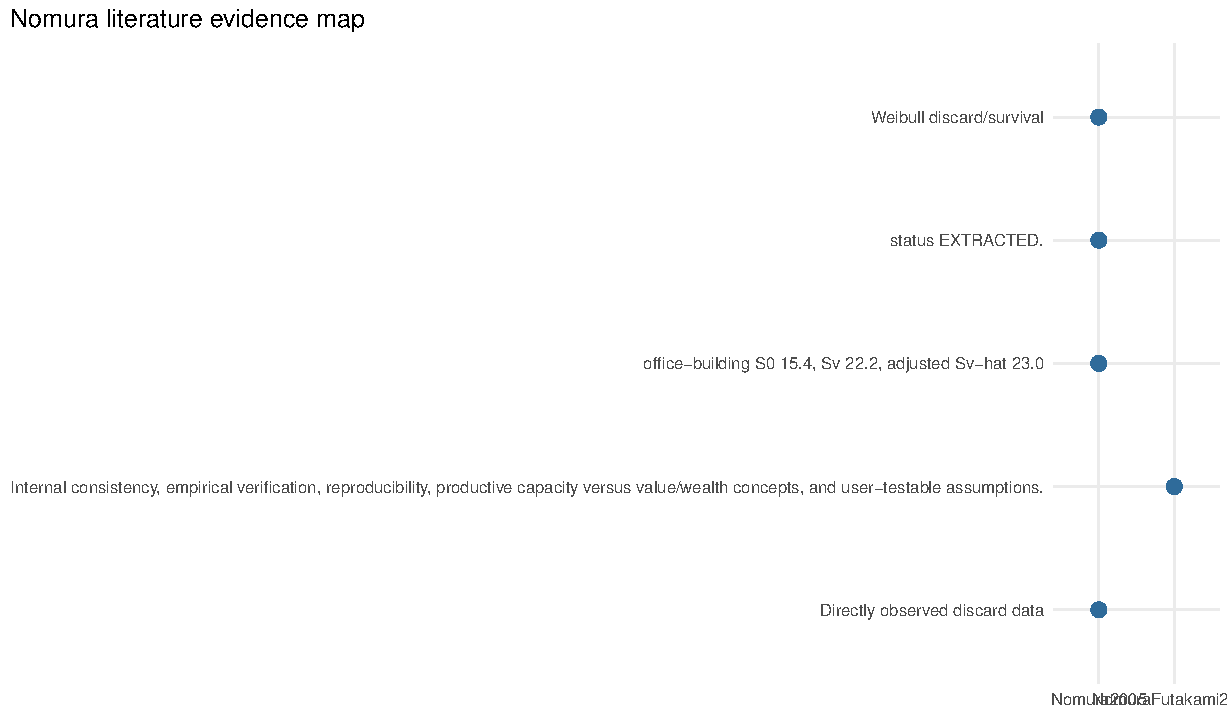
\includegraphics[width=0.92\linewidth]{../figures/D09_S_fig01_Nomura_literature_evidence_map.pdf}\caption{Literature evidence map. This figure summarizes the bounded use of Nomura 2005 and Nomura-Futakami 2005. The sources motivate report-only sensitivity and do not impose a U.S. NRC benchmark.}\end{figure}\FloatBarrier
\section{Capital Concepts: Gross, Productive, Net, Discard, Decay, and Disposal}
The literature distinguishes gross, productive, and net or wealth capital concepts and separates discard, retirement, scrapping, disposal, and decay. D09-S uses gross surviving GPIM stocks as the inspected object while keeping pKN valuation and current-cost accounting separate.
\section{Baseline GPIM Architecture and Equations}
\begin{align} I^{R}_{j,t} &= \frac{I^{C}_{j,t}}{p^{K}_{j,t}/100}\\ K^{R}_{j,t}(L_j,\alpha_j) &= \sum_{a=0}^{A} s_j(a;L_j,\alpha_j) I^{R}_{j,t-a}\\ K^{C}_{j,t}(L_j,\alpha_j) &= K^{R}_{j,t}(L_j,\alpha_j)\frac{p^{K}_{j,t}}{100}\\ K^{R}_{cap,t} &= K^{R}_{ME,t}+K^{R}_{NRC,t}\\ K^{C}_{cap,t} &= K^{C}_{ME,t}+K^{C}_{NRC,t}\\ X^{index,b}_{t} &= 100\times\frac{X_t}{X_b}\end{align}
All sensitivity stocks, ratios, and indices are report-only inspection artifacts. They are not D06 baseline replacements and are not D10 model transformations.
\section{Service-Life Sensitivity Design}
ME uses conservative cases around the locked L=14 profile. NRC uses the D09-R design range: L=23 as a Nomura-office comparison, L=40, L=50, L=60, and shape checks at alpha 1.2 and 2.0. No total capital, IPP, residential, or government transportation object is constructed.
\section{Survival Profiles for ME and NRC}
\begin{figure}[H]\centering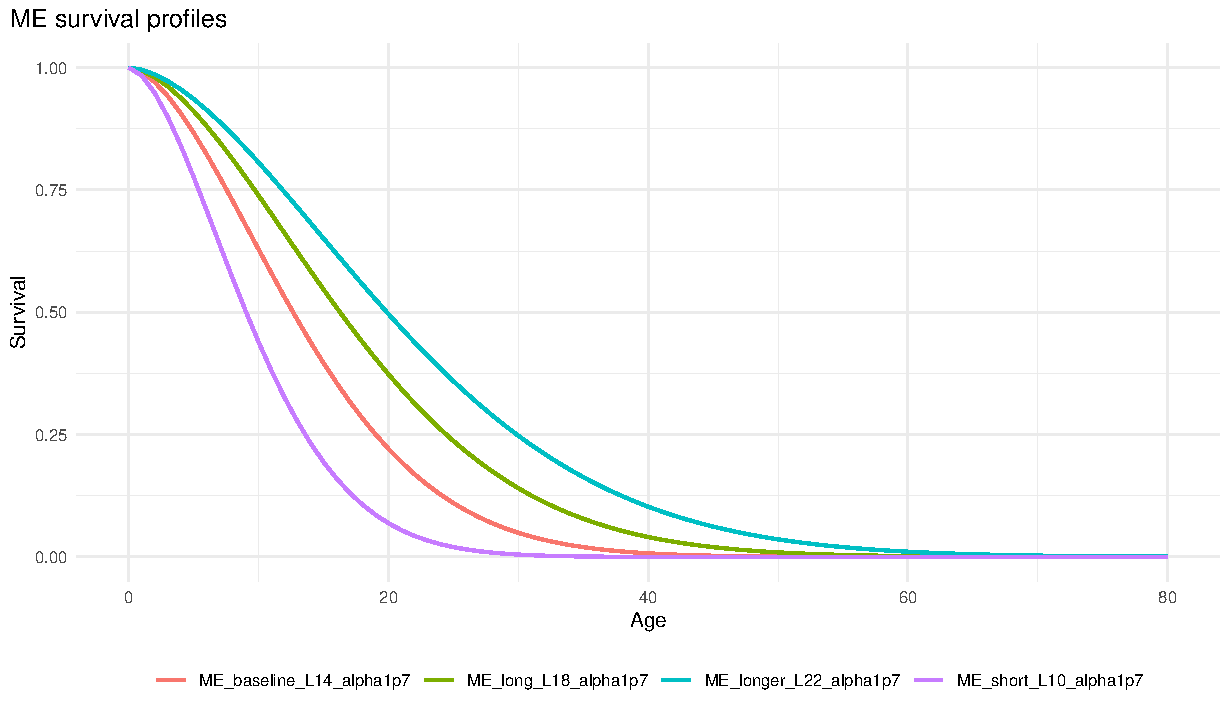
\includegraphics[width=0.92\linewidth]{../figures/D09_S_fig02_ME_survival_profiles.pdf}\caption{ME survival profiles. These report-only survival profiles vary ME service life around the D06 baseline while preserving alpha=1.7.}\end{figure}\FloatBarrier
\begin{figure}[H]\centering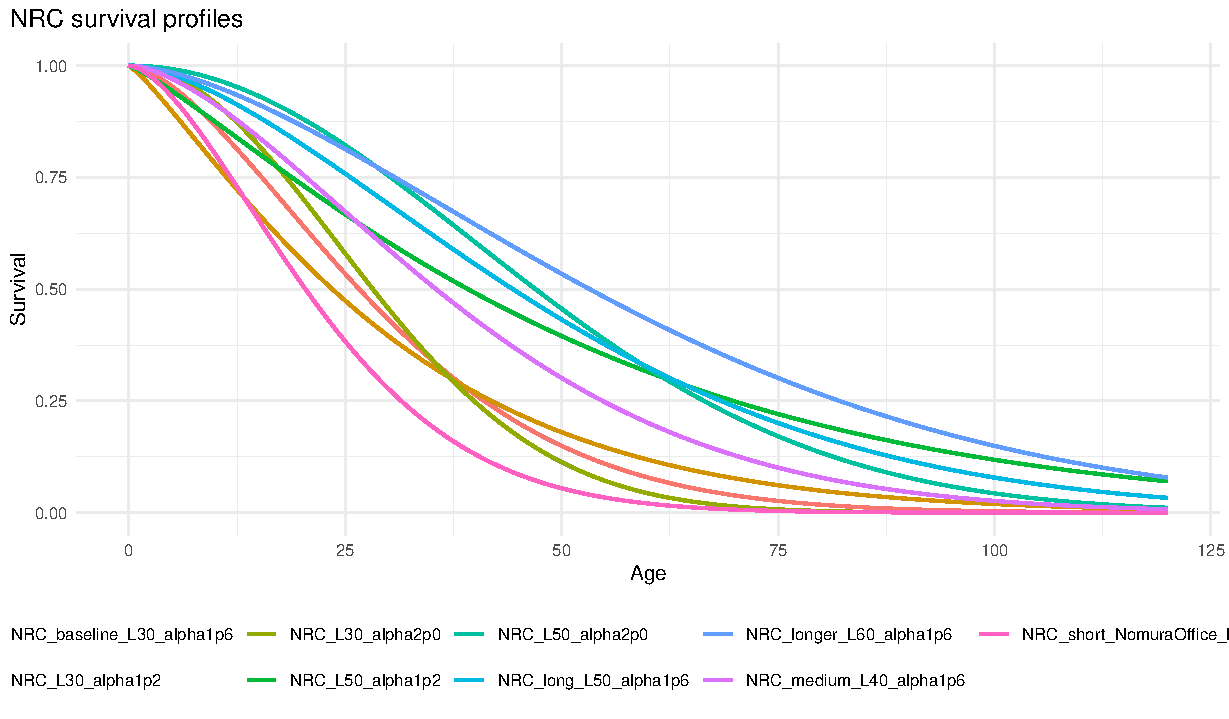
\includegraphics[width=0.92\linewidth]{../figures/D09_S_fig03_NRC_survival_profiles.pdf}\caption{NRC survival profiles. These report-only profiles include the D06 baseline, the Nomura-office comparison, longer-life robustness cases, and shape checks.}\end{figure}\FloatBarrier
\section{Warmup, Initialization, and Inherited-Vintage Risk}
The D06 convention is preserved: no inherited pre-price capital stock is invented. Longer NRC lives reduce late-sample decline mechanically but make the missing inherited-vintage problem more severe because NRC starts in 1931 and analysis begins in 1947.
\begin{figure}[H]\centering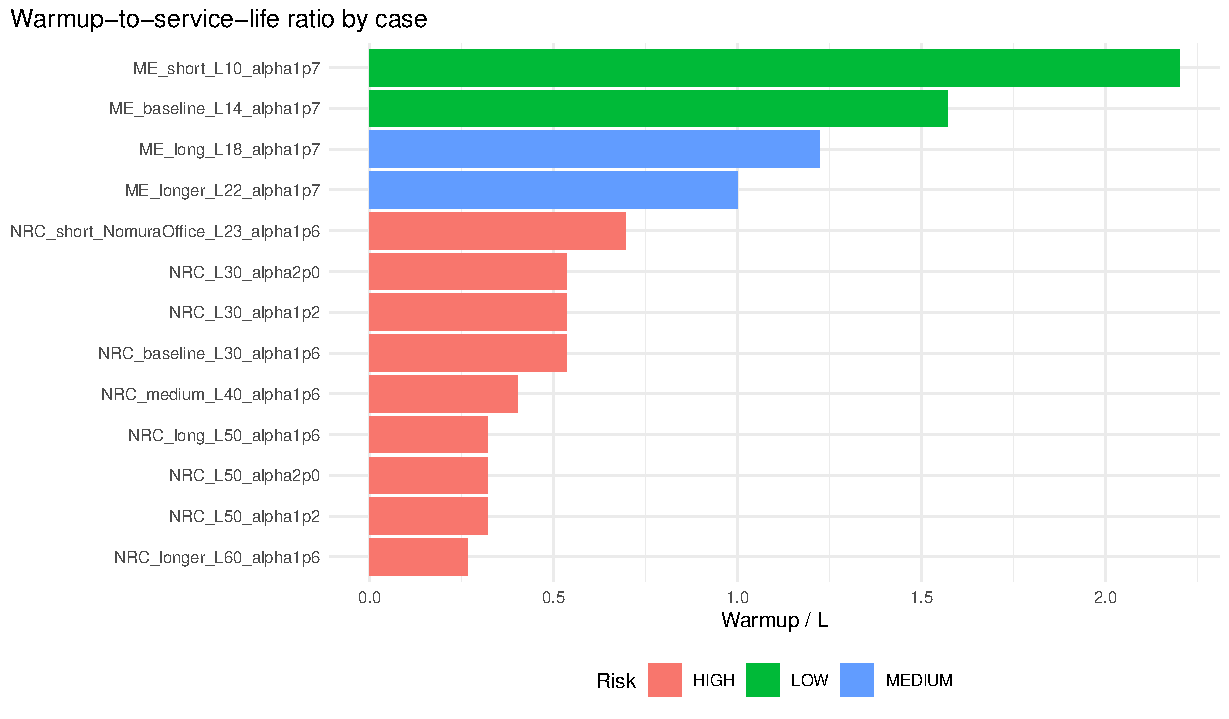
\includegraphics[width=0.92\linewidth]{../figures/D09_S_fig04_warmup_to_L_ratio_by_case.pdf}\caption{Warmup-to-L ratio by case. Longer NRC service-life cases are flagged as higher initialization risk; this risk is review-required but not blocking because identity checks pass.}\end{figure}\FloatBarrier
\section{ME Gross GPIM Sensitivity Results}
ME sensitivity is visually stable over the conservative range. The ME baseline remains defensible for D10 planning because the alternative service lives do not overturn the qualitative path.
\begin{figure}[H]\centering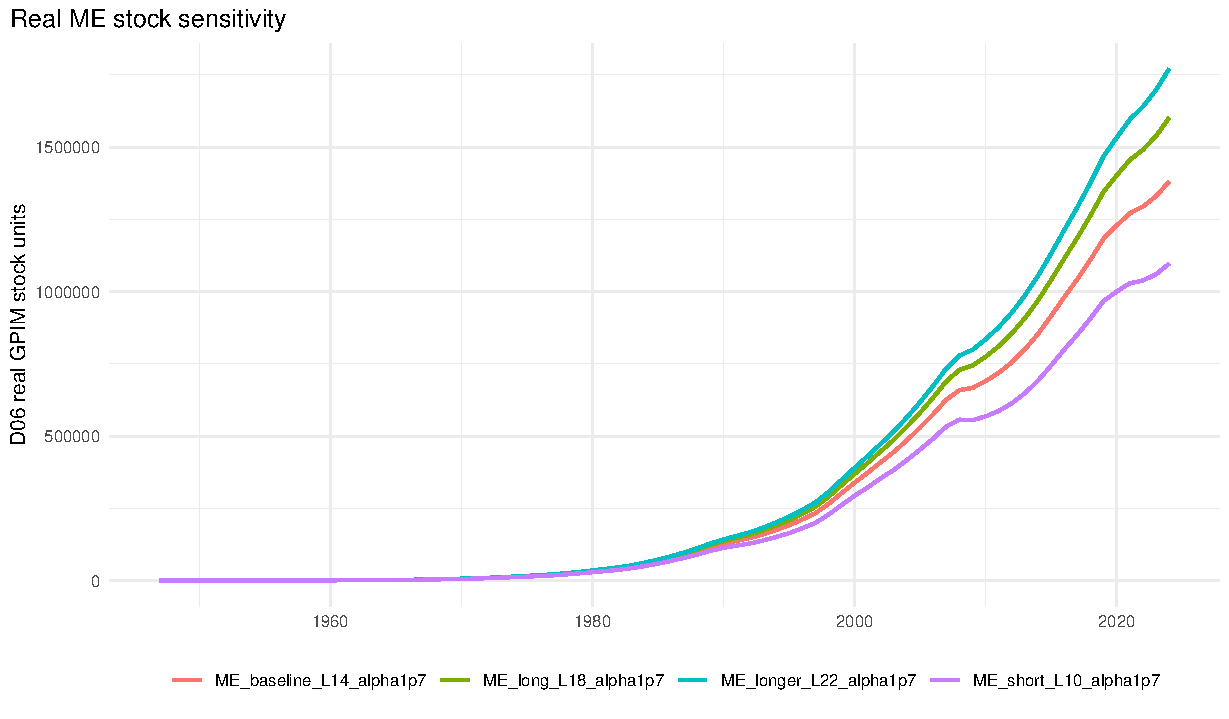
\includegraphics[width=0.92\linewidth]{../figures/D09_S_fig05_real_ME_stock_sensitivity.pdf}\caption{Real ME stock sensitivity. Report-only ME gross GPIM stocks are compared against the D06 baseline; no sensitivity stock is a source-of-truth replacement.}\end{figure}\FloatBarrier
\begin{figure}[H]\centering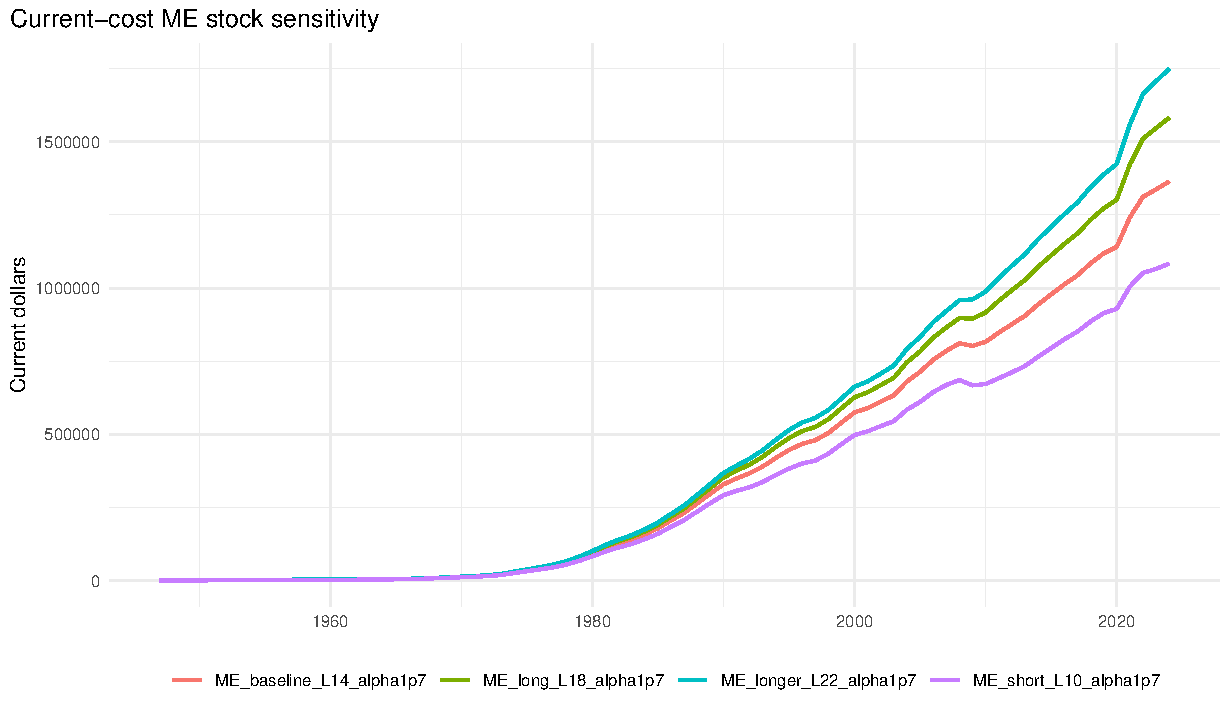
\includegraphics[width=0.92\linewidth]{../figures/D09_S_fig06_current_ME_stock_sensitivity.pdf}\caption{Current-cost ME stock sensitivity. Current-cost sensitivity combines report-only real ME stock cases with the unchanged D06 pKN path.}\end{figure}\FloatBarrier
\begin{figure}[H]\centering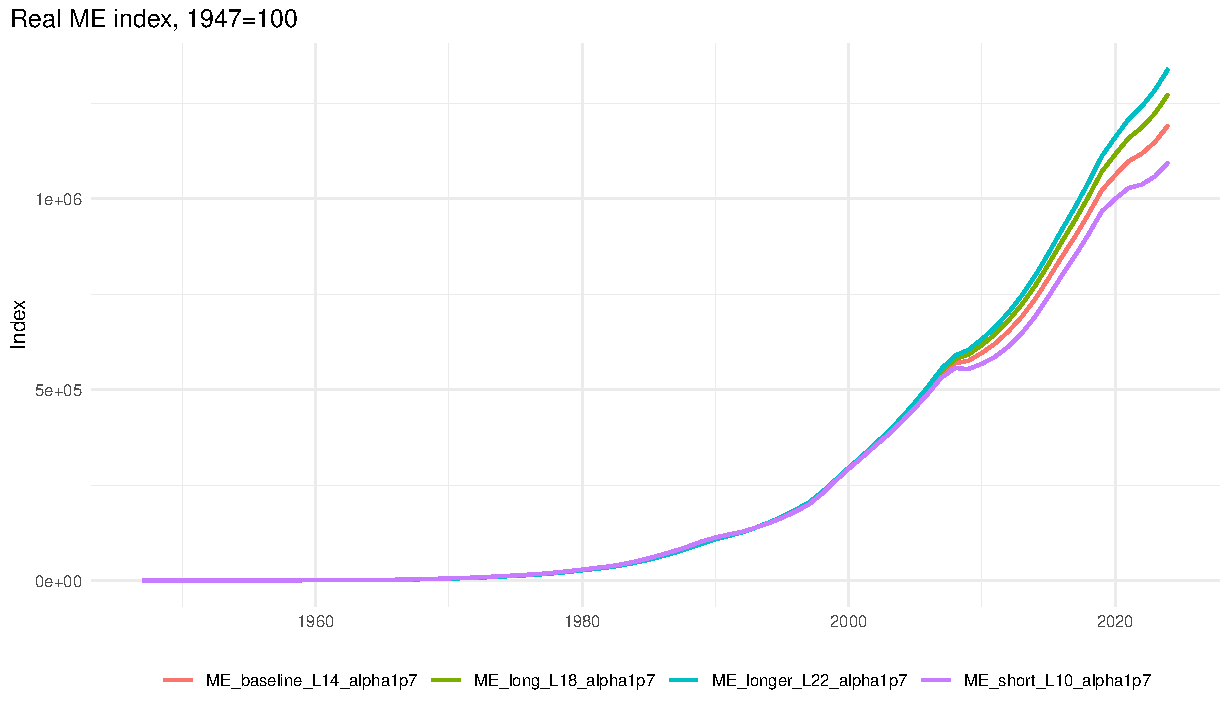
\includegraphics[width=0.92\linewidth]{../figures/D09_S_fig07_real_ME_index_1947_100_sensitivity.pdf}\caption{Real ME index, 1947=100. The index is a report-only visual normalization.}\end{figure}\FloatBarrier
\begin{figure}[H]\centering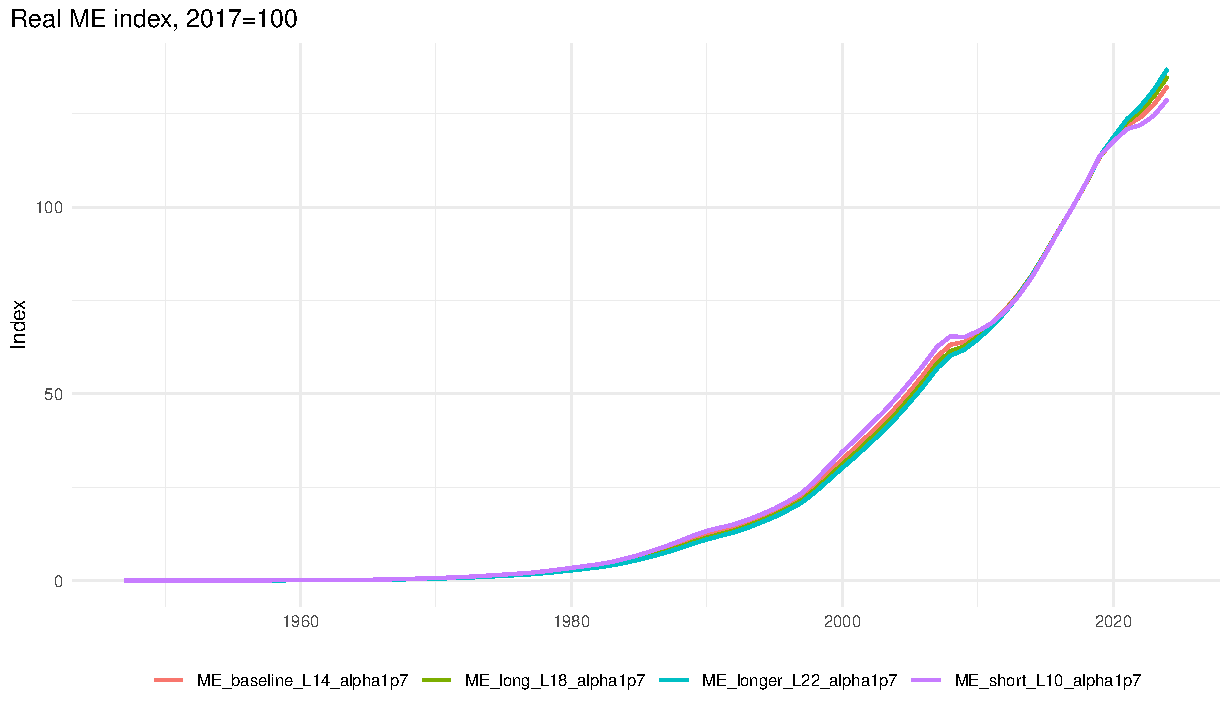
\includegraphics[width=0.92\linewidth]{../figures/D09_S_fig08_real_ME_index_2017_100_sensitivity.pdf}\caption{Real ME index, 2017=100. The index is not a model transformation.}\end{figure}\FloatBarrier
\section{NRC Gross GPIM Sensitivity Results}
The baseline NRC peak-to-latest change is -44.3 percent; the L50 case is -22 percent. Longer lives reduce the decline but increase warmup fragility, so the verdict is proceed with an NRC robustness flag rather than replace the D06 baseline.
\begin{figure}[H]\centering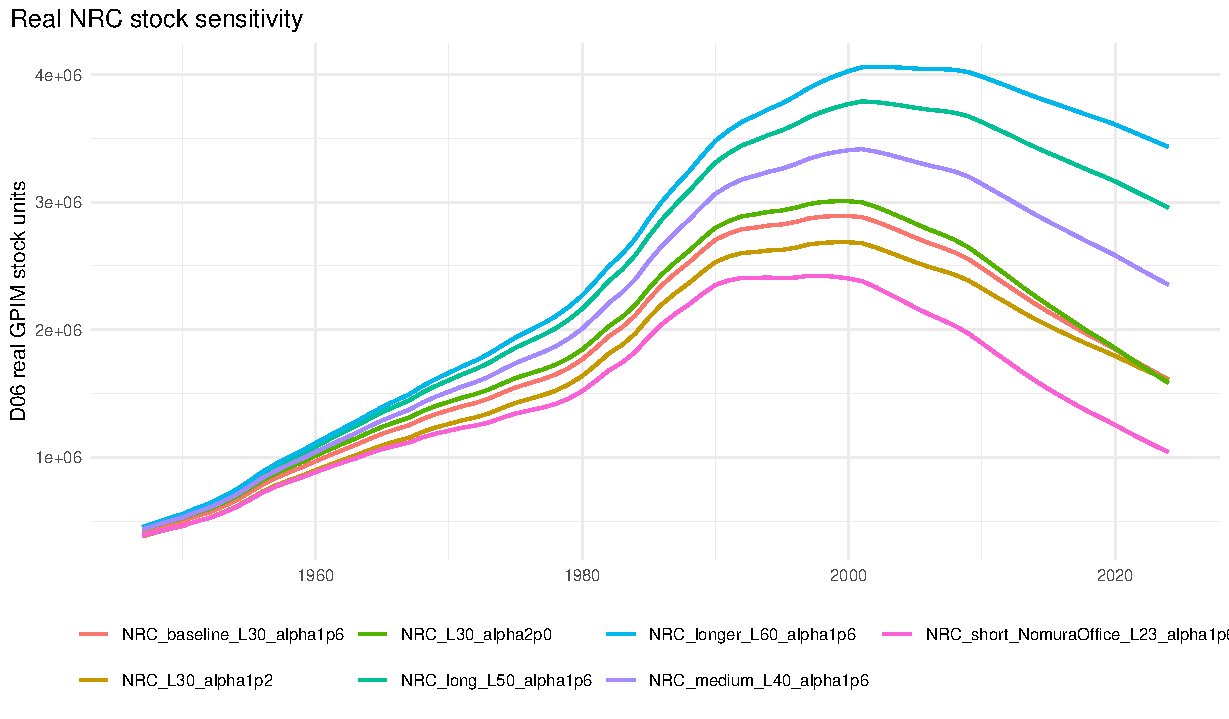
\includegraphics[width=0.92\linewidth]{../figures/D09_S_fig09_real_NRC_stock_sensitivity.pdf}\caption{Real NRC stock sensitivity. Longer service lives reduce the late-sample decline but do not become D06 baseline replacements.}\end{figure}\FloatBarrier
\begin{figure}[H]\centering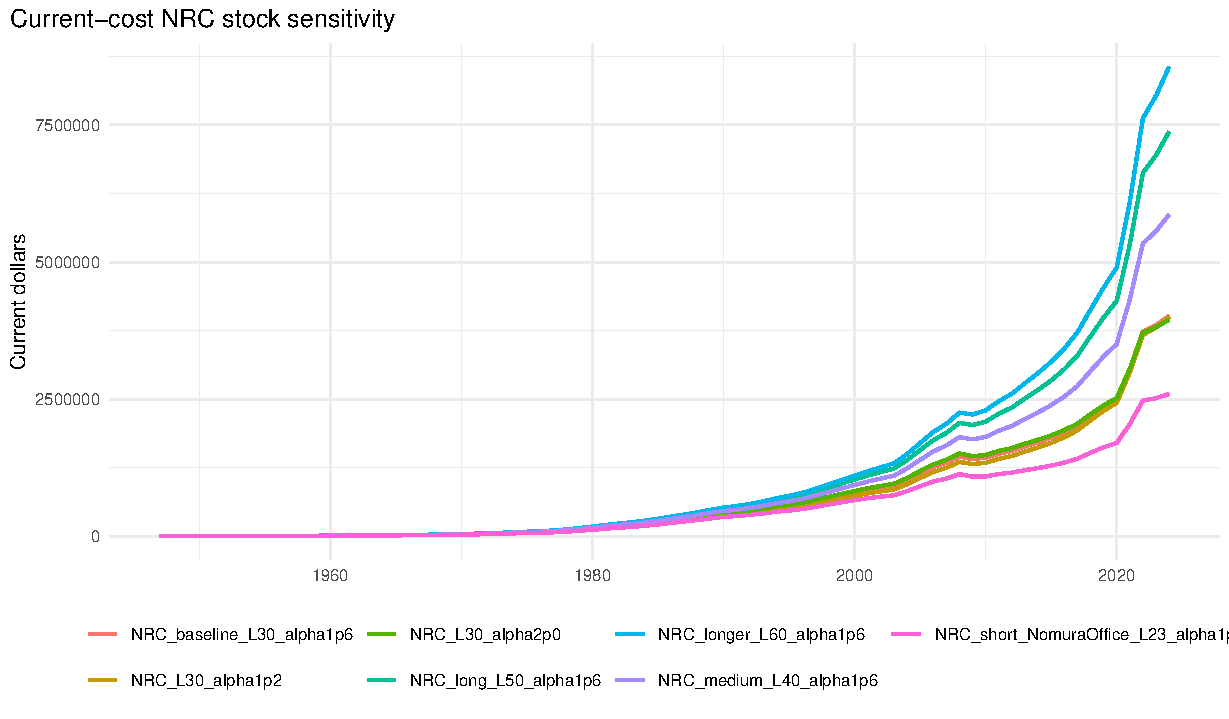
\includegraphics[width=0.92\linewidth]{../figures/D09_S_fig10_current_NRC_stock_sensitivity.pdf}\caption{Current-cost NRC stock sensitivity. Current-cost paths mix real sensitivity and unchanged pKN valuation.}\end{figure}\FloatBarrier
\begin{figure}[H]\centering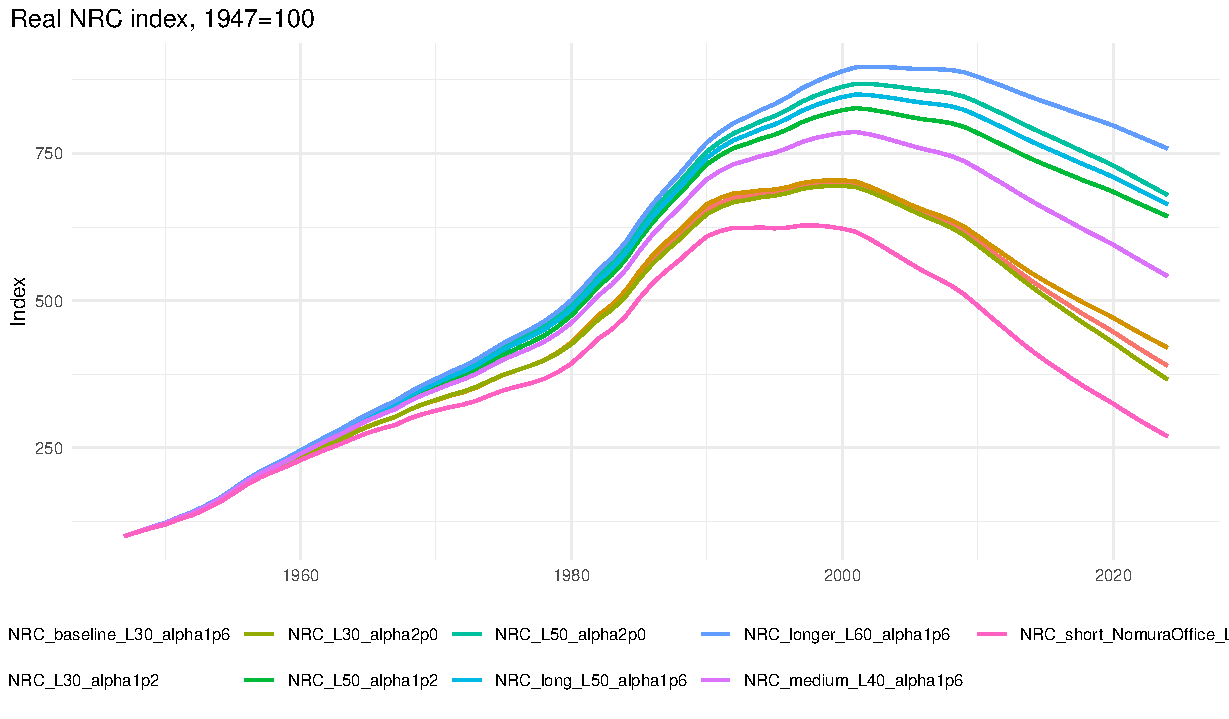
\includegraphics[width=0.92\linewidth]{../figures/D09_S_fig11_real_NRC_index_1947_100_sensitivity.pdf}\caption{Real NRC index, 1947=100. The Nomura-office comparison is shorter than the D06 NRC baseline and is not a U.S. NRC benchmark.}\end{figure}\FloatBarrier
\begin{figure}[H]\centering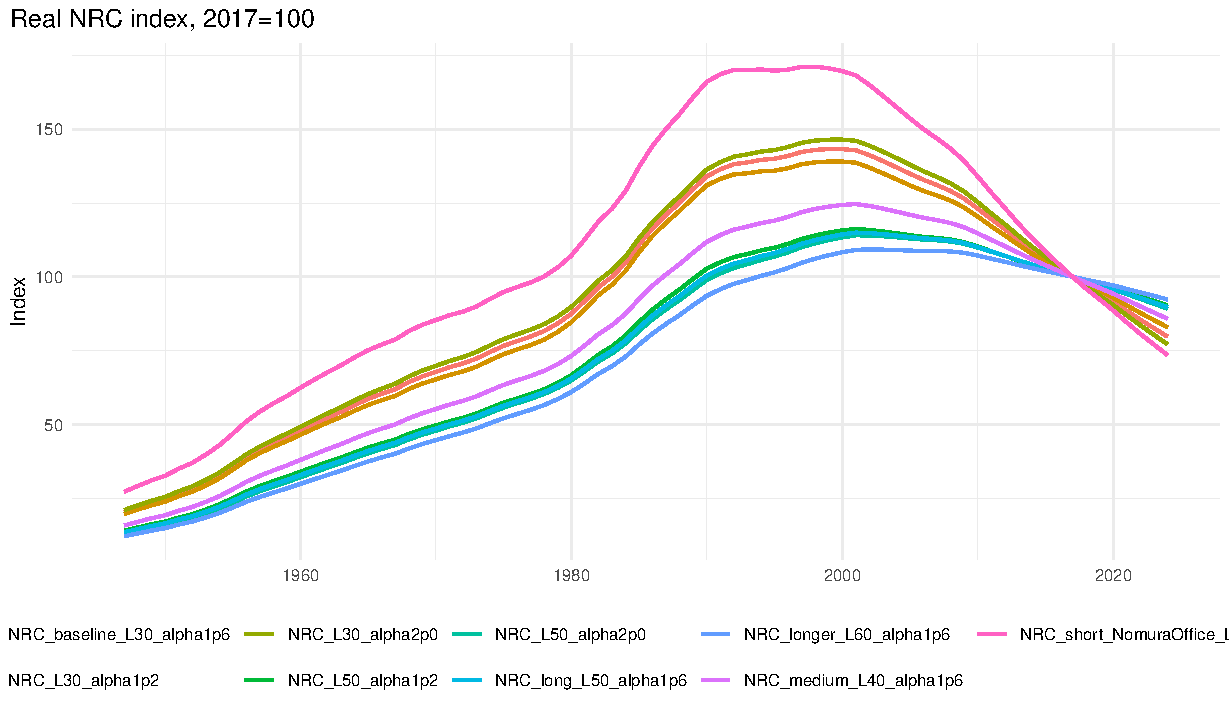
\includegraphics[width=0.92\linewidth]{../figures/D09_S_fig12_real_NRC_index_2017_100_sensitivity.pdf}\caption{Real NRC index, 2017=100. The visual normalization is report-only.}\end{figure}\FloatBarrier
\section{Capacity-Capital Sensitivity: ME+NRC}
Capacity sensitivity combines ME and NRC cases without constructing total capital. The principal comparison holds ME at baseline and varies NRC service life.
\begin{figure}[H]\centering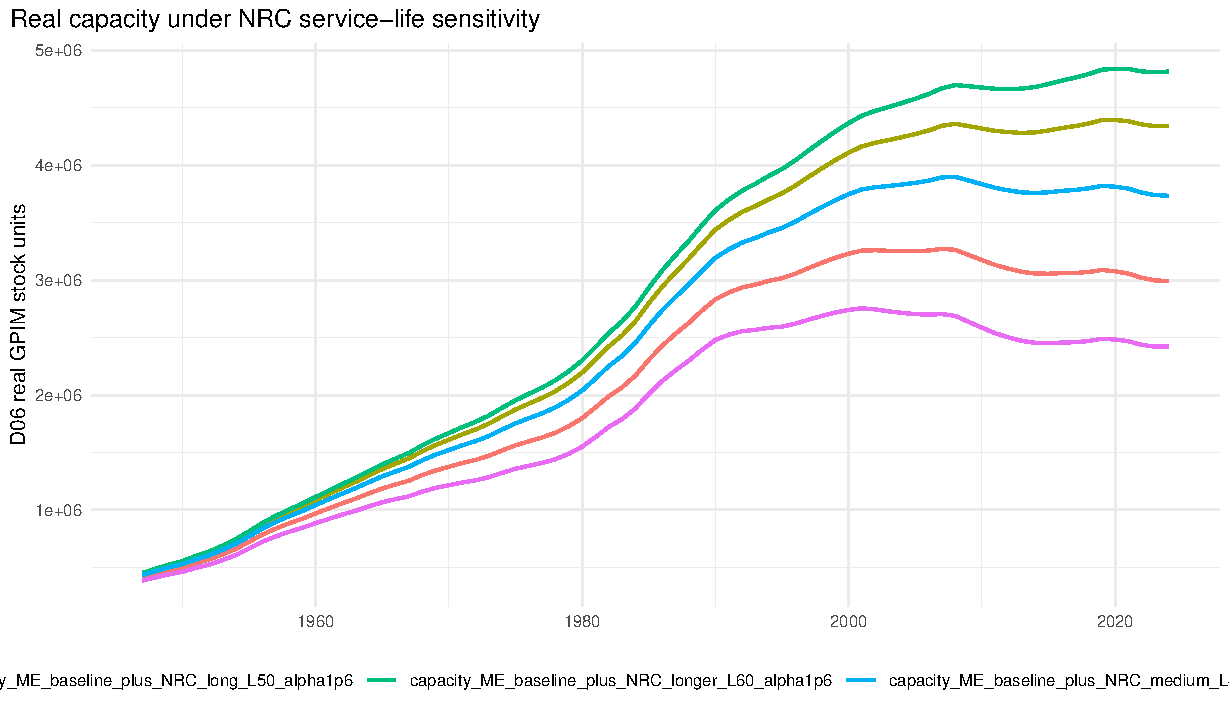
\includegraphics[width=0.92\linewidth]{../figures/D09_S_fig13_real_capacity_NRC_life_sensitivity.pdf}\caption{Real capacity under NRC service-life sensitivity. Capacity remains ME plus NRC only.}\end{figure}\FloatBarrier
\begin{figure}[H]\centering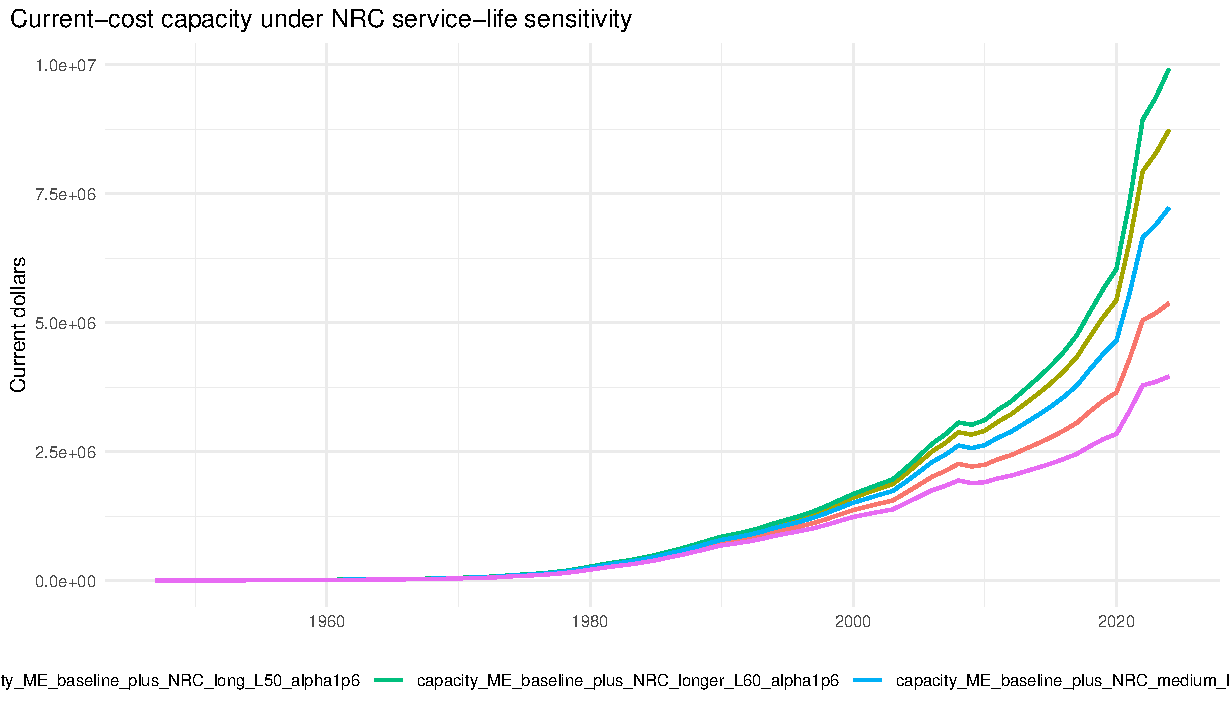
\includegraphics[width=0.92\linewidth]{../figures/D09_S_fig14_current_capacity_NRC_life_sensitivity.pdf}\caption{Current-cost capacity under NRC service-life sensitivity. The pKN path is unchanged.}\end{figure}\FloatBarrier
\begin{figure}[H]\centering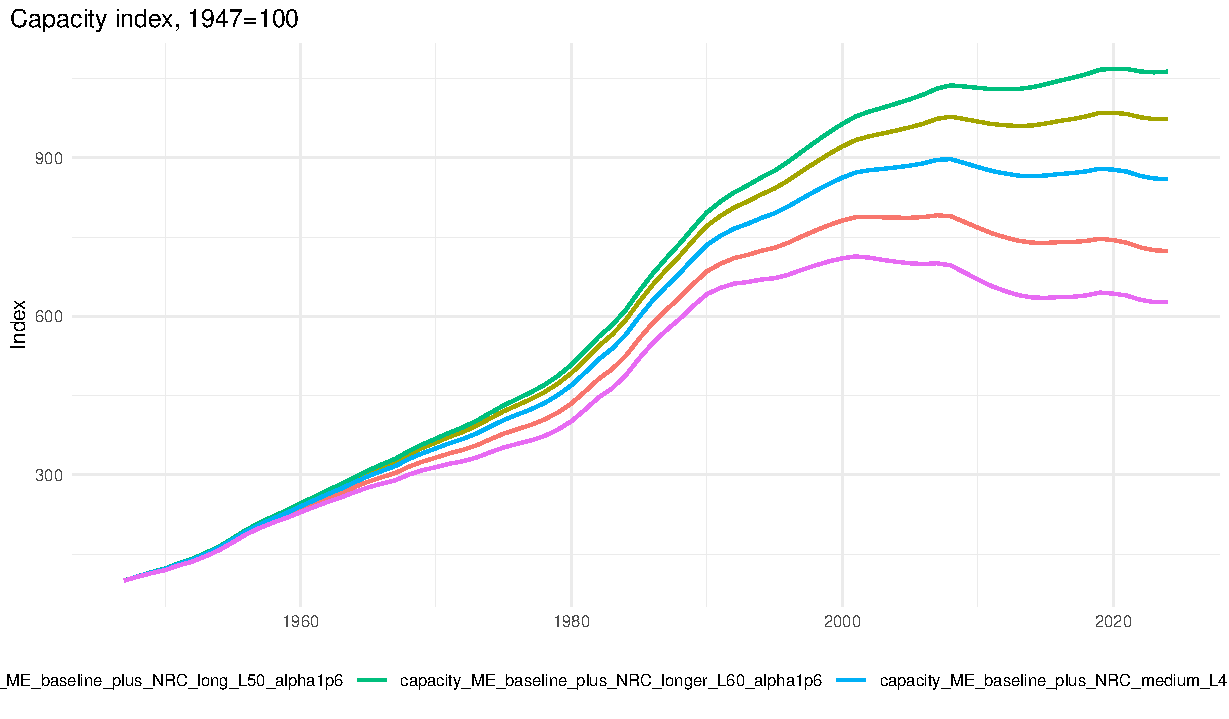
\includegraphics[width=0.92\linewidth]{../figures/D09_S_fig15_capacity_index_1947_100_NRC_sensitivity.pdf}\caption{Capacity index, 1947=100. Report-only visual normalization.}\end{figure}\FloatBarrier
\begin{figure}[H]\centering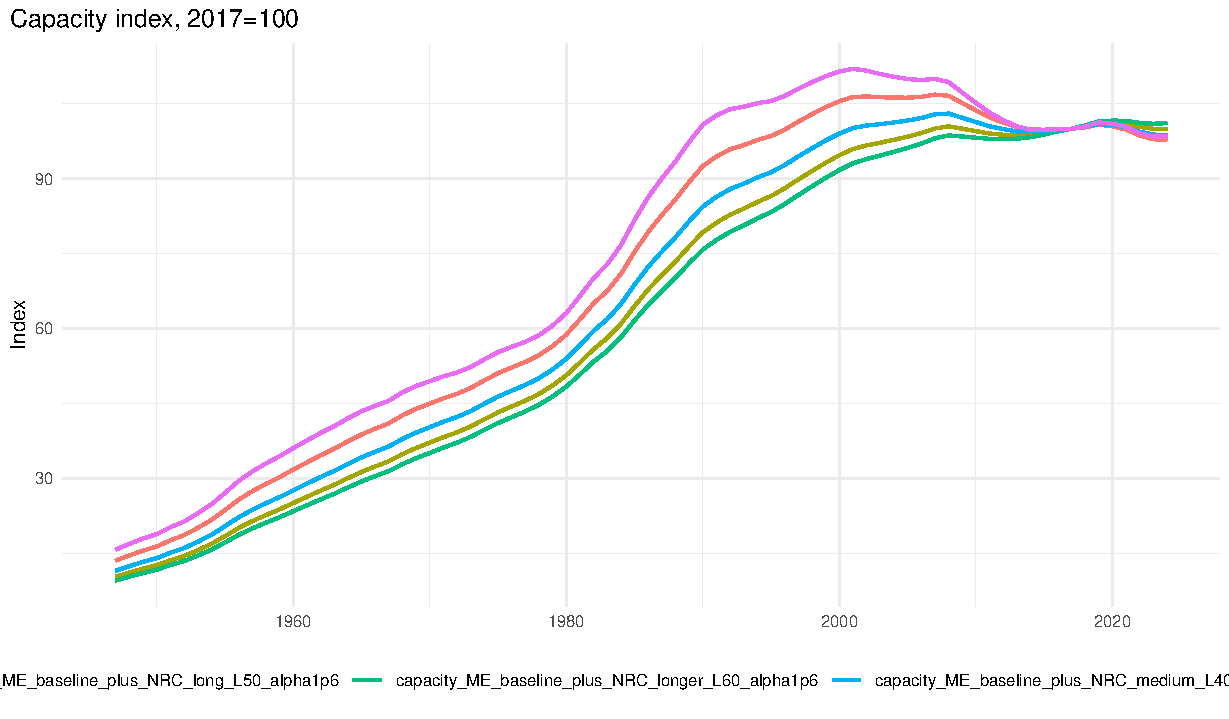
\includegraphics[width=0.92\linewidth]{../figures/D09_S_fig16_capacity_index_2017_100_NRC_sensitivity.pdf}\caption{Capacity index, 2017=100. Report-only visual normalization.}\end{figure}\FloatBarrier
\section{ME/NRC Composition and Mechanization Sensitivity}
Composition diagnostics show how service-life choices shift the ME/NRC balance. These ratios are not q and are not model-ready.
\begin{figure}[H]\centering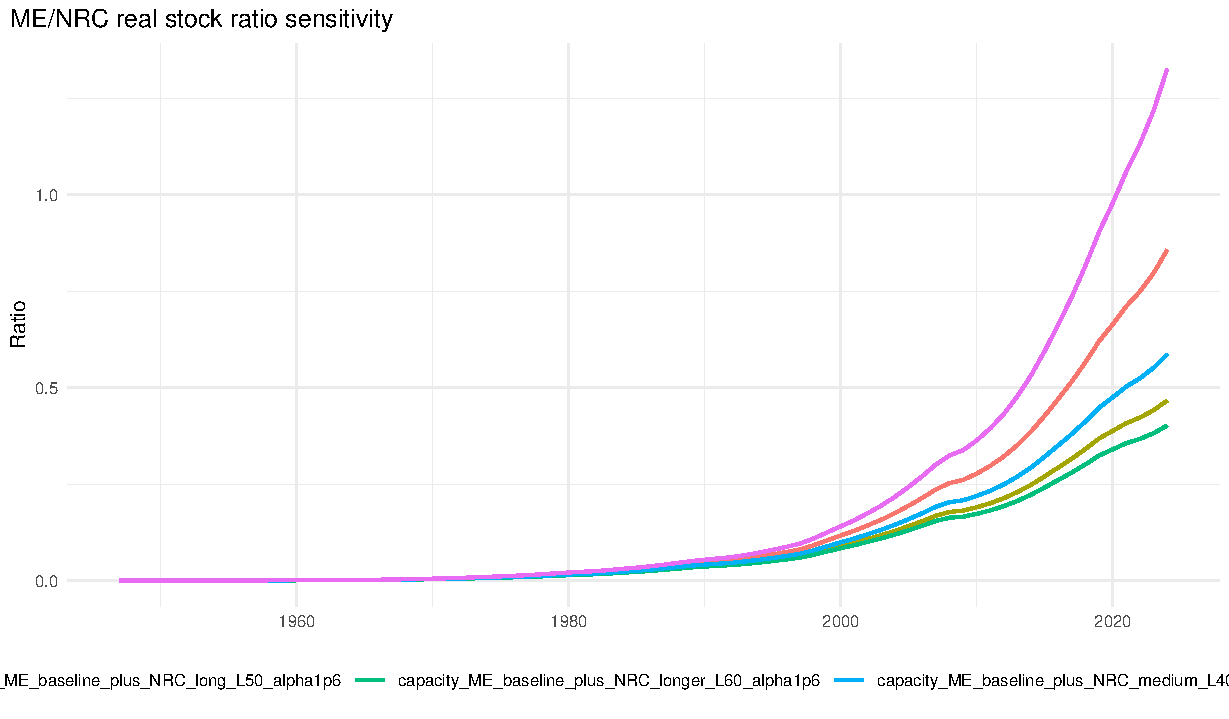
\includegraphics[width=0.92\linewidth]{../figures/D09_S_fig17_ME_over_NRC_real_stock_ratio_sensitivity.pdf}\caption{ME/NRC real stock ratio sensitivity. Report-only composition diagnostic.}\end{figure}\FloatBarrier
\begin{figure}[H]\centering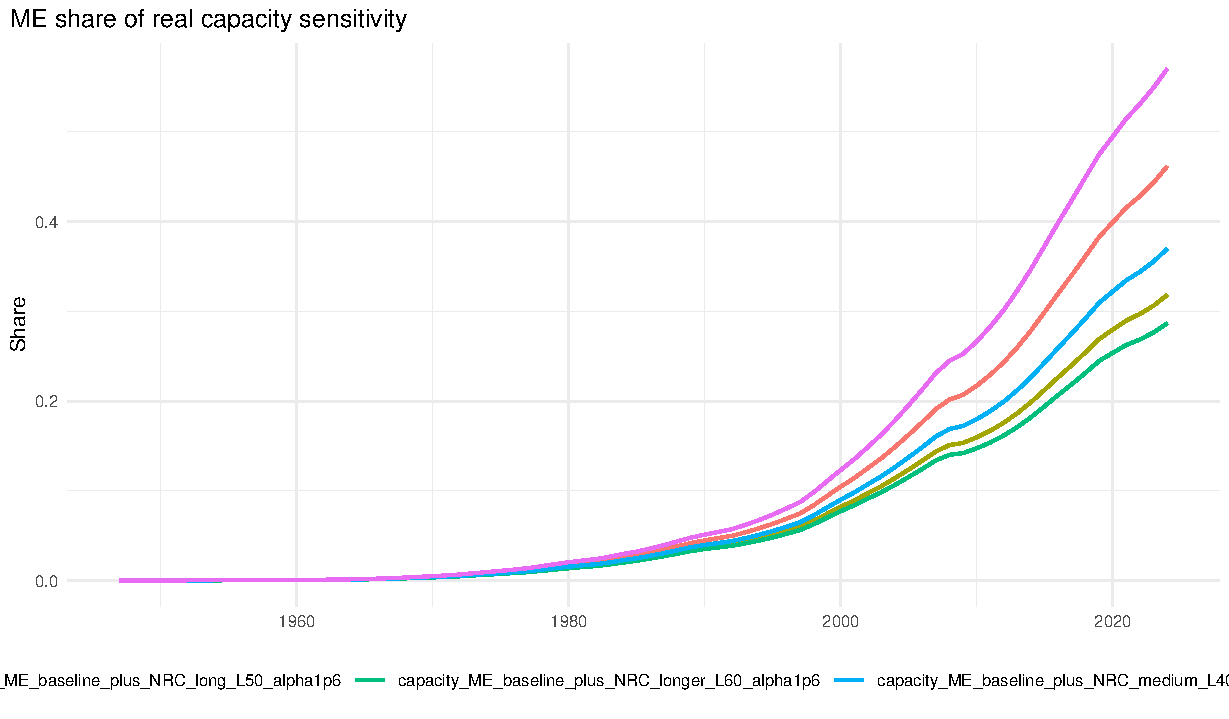
\includegraphics[width=0.92\linewidth]{../figures/D09_S_fig18_ME_share_real_capacity_sensitivity.pdf}\caption{ME share of real capacity sensitivity. Report-only composition diagnostic.}\end{figure}\FloatBarrier
\section{Output-Capital Visual Sensitivity}
Output-capital relations are inspected visually only. D09-S runs no regressions, stationarity tests, integration tests, or cointegration tests.
\begin{figure}[H]\centering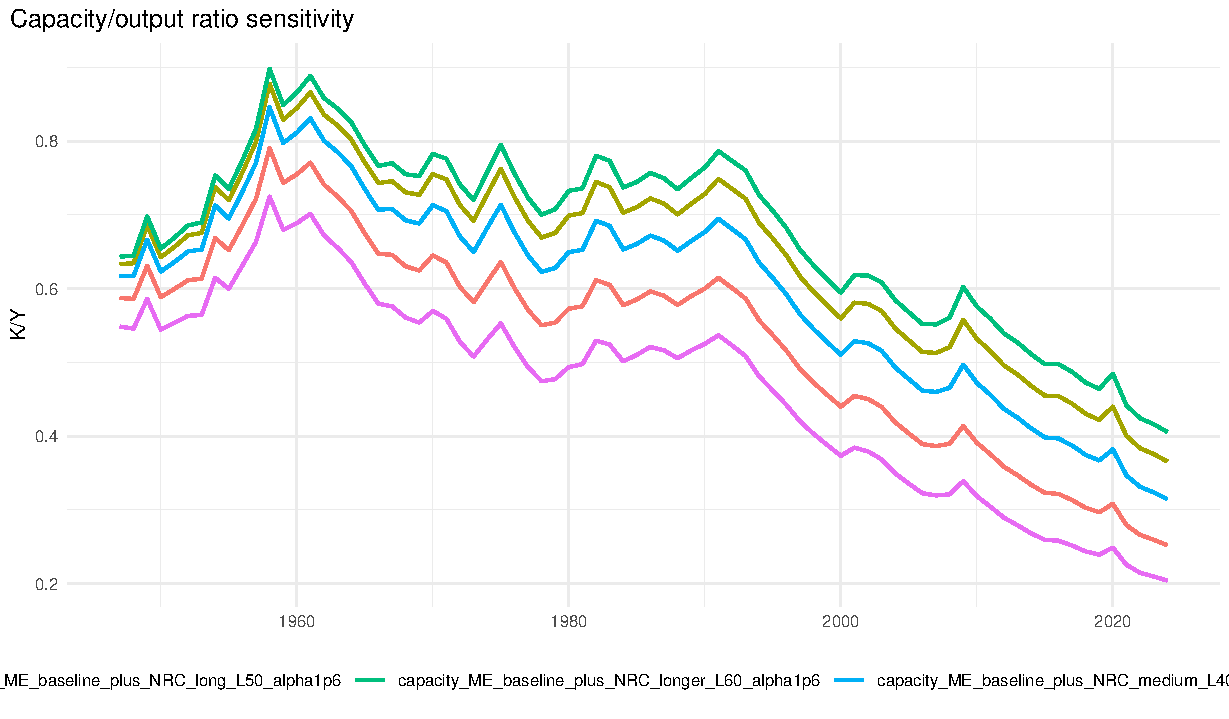
\includegraphics[width=0.92\linewidth]{../figures/D09_S_fig19_capacity_output_ratio_sensitivity.pdf}\caption{Capacity/output ratio sensitivity. Report-only visual inspection.}\end{figure}\FloatBarrier
\begin{figure}[H]\centering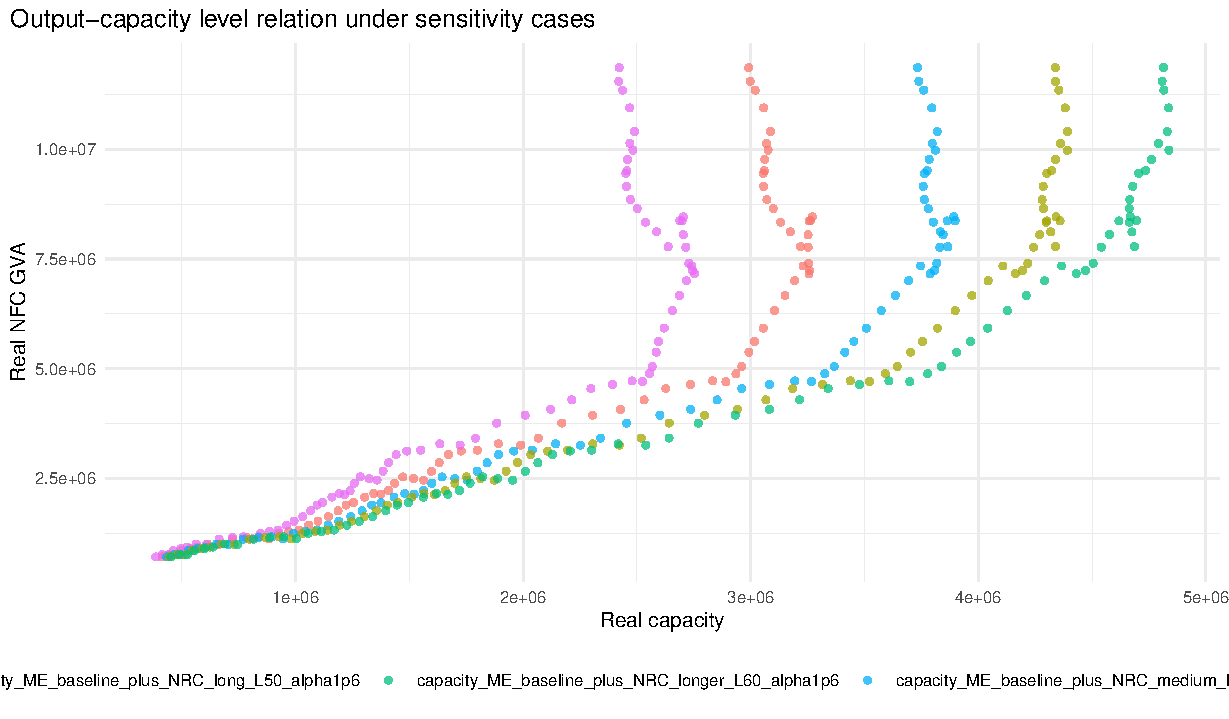
\includegraphics[width=0.92\linewidth]{../figures/D09_S_fig20_output_capacity_level_relation_sensitivity.pdf}\caption{Output-capacity level relation sensitivity. The scatter contains no fitted line.}\end{figure}\FloatBarrier
\section{Stock-Flow and Current-Cost Identity Audits}
Identity audits pass across the report-only cases. This supports proceeding with a robustness flag rather than blocking the pipeline.
\begin{figure}[H]\centering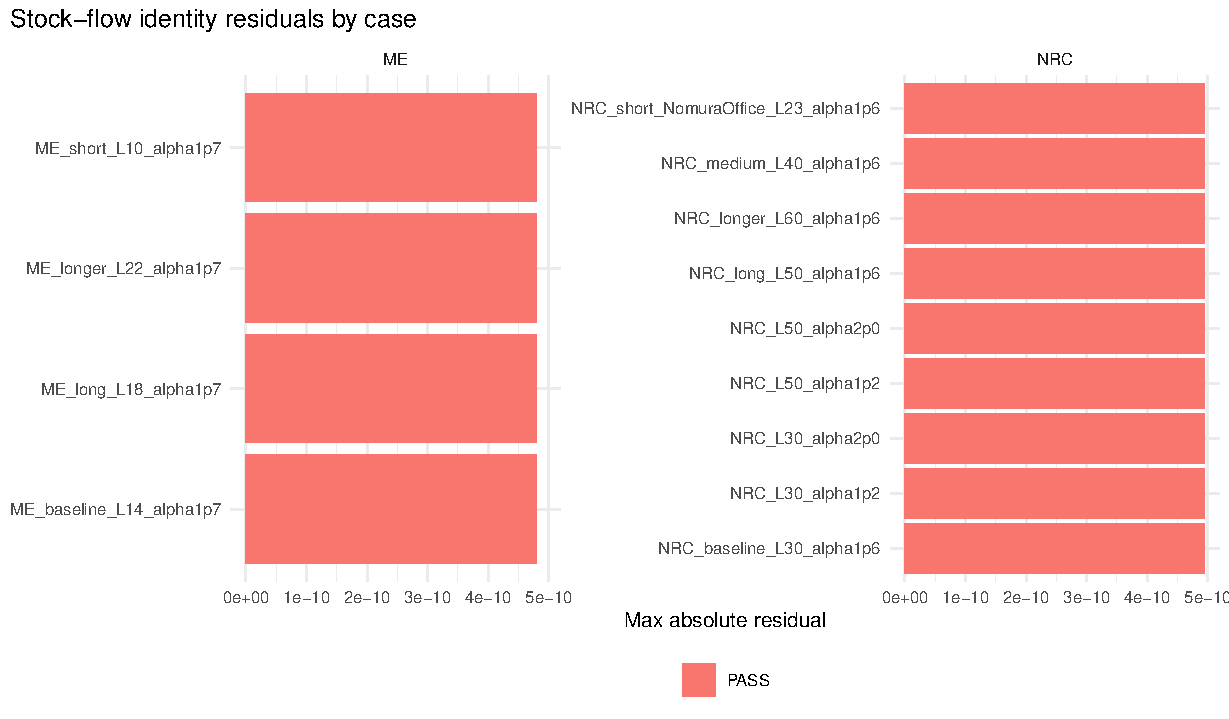
\includegraphics[width=0.92\linewidth]{../figures/D09_S_fig24_stock_flow_identity_residuals_by_case.pdf}\caption{Stock-flow identity residuals by case. The guarded real-investment identity remains numerically coherent.}\end{figure}\FloatBarrier
\begin{figure}[H]\centering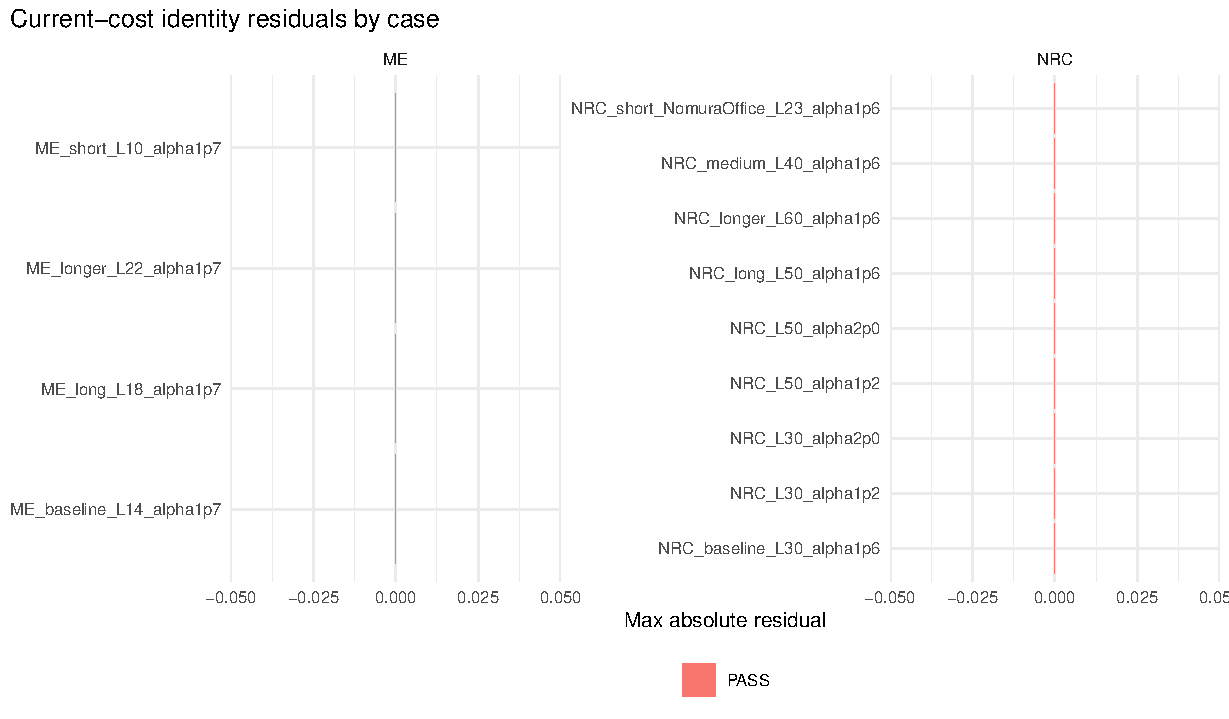
\includegraphics[width=0.92\linewidth]{../figures/D09_S_fig25_current_cost_identity_residuals_by_case.pdf}\caption{Current-cost identity residuals by case. Current-cost stocks equal real stocks times unchanged pKN.}\end{figure}\FloatBarrier
\begin{figure}[H]\centering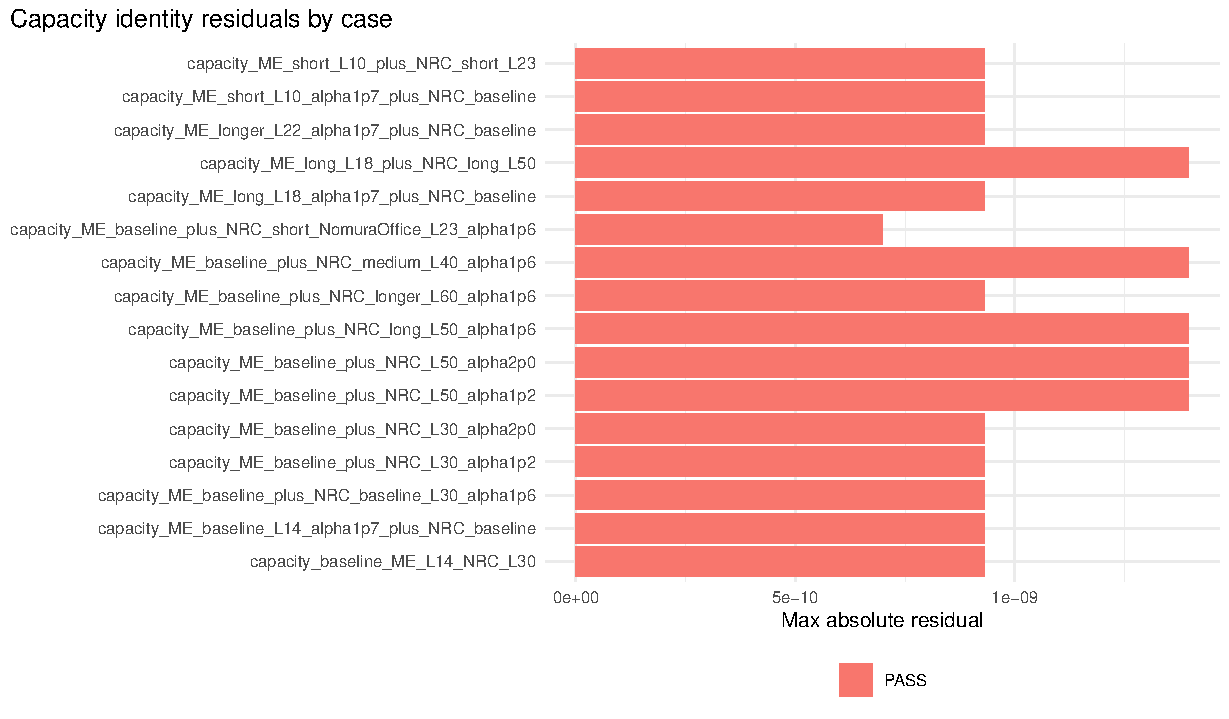
\includegraphics[width=0.92\linewidth]{../figures/D09_S_fig26_capacity_identity_residuals_by_case.pdf}\caption{Capacity identity residuals by case. Capacity equals ME plus NRC for every capacity case.}\end{figure}\FloatBarrier
\section{Interpretation of NRC Decline Across Sensitivity Cases}
If longer NRC service lives eliminate or reduce the real NRC decline, the baseline path is service-life sensitive. D09-S measures that reduction and keeps the warning attached to D10 planning. If the L=23 Nomura-office comparison produces a stronger decline, that is evidence that Japanese office-building estimates alone do not justify lengthening U.S. NRC survival.
\begin{figure}[H]\centering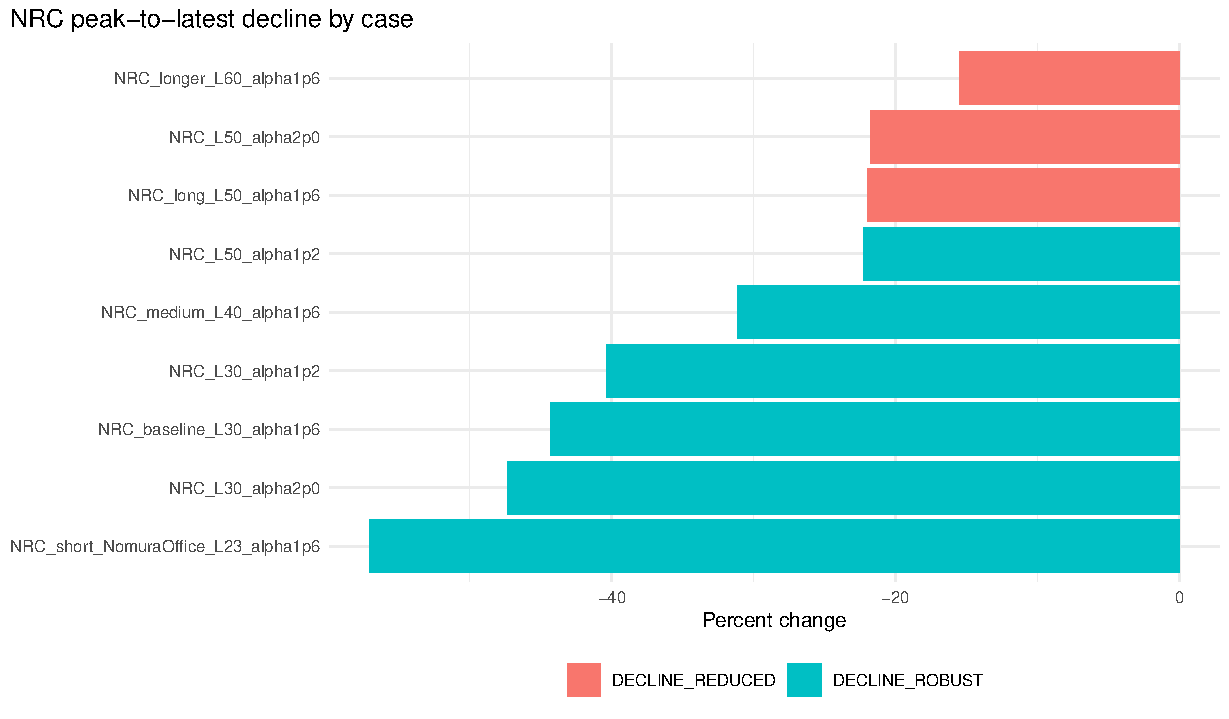
\includegraphics[width=0.92\linewidth]{../figures/D09_S_fig21_NRC_peak_to_latest_decline_by_case.pdf}\caption{NRC peak-to-latest decline by case. This is the measured basis for the NRC sensitivity interpretation.}\end{figure}\FloatBarrier
\begin{figure}[H]\centering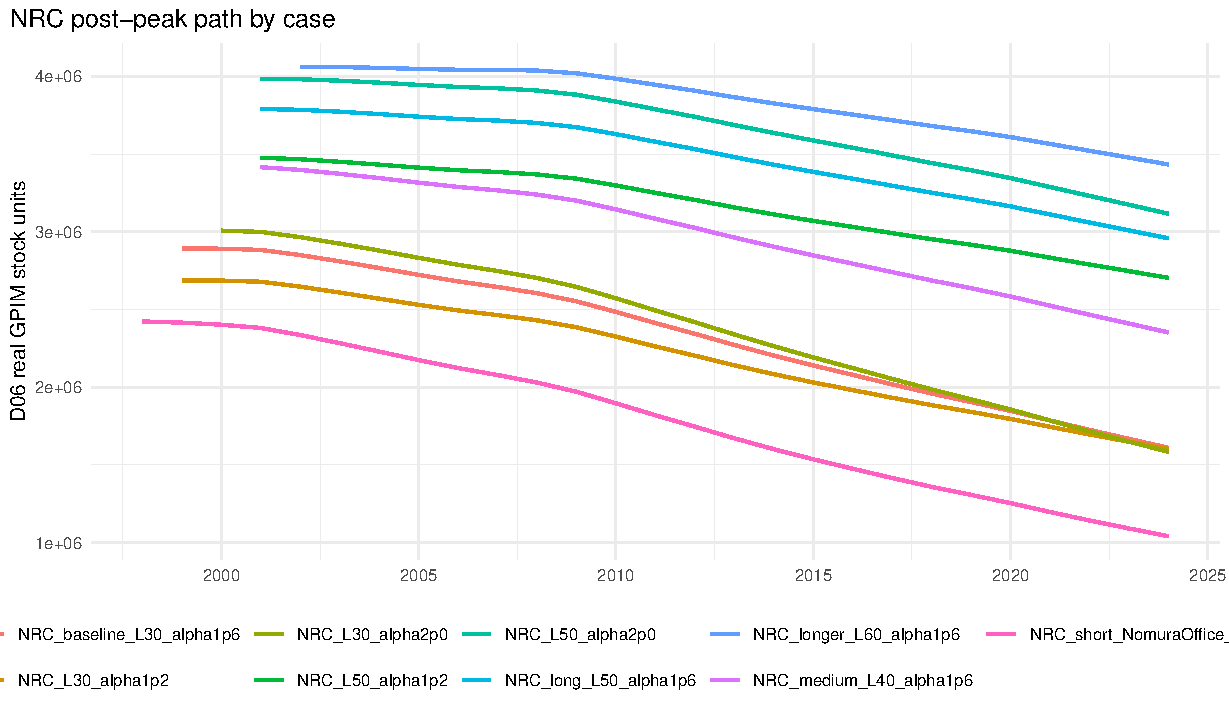
\includegraphics[width=0.92\linewidth]{../figures/D09_S_fig22_NRC_post_peak_path_by_case.pdf}\caption{NRC post-peak path by case. Longer-life cases reduce the late-sample decline but raise initialization review risk.}\end{figure}\FloatBarrier
\begin{figure}[H]\centering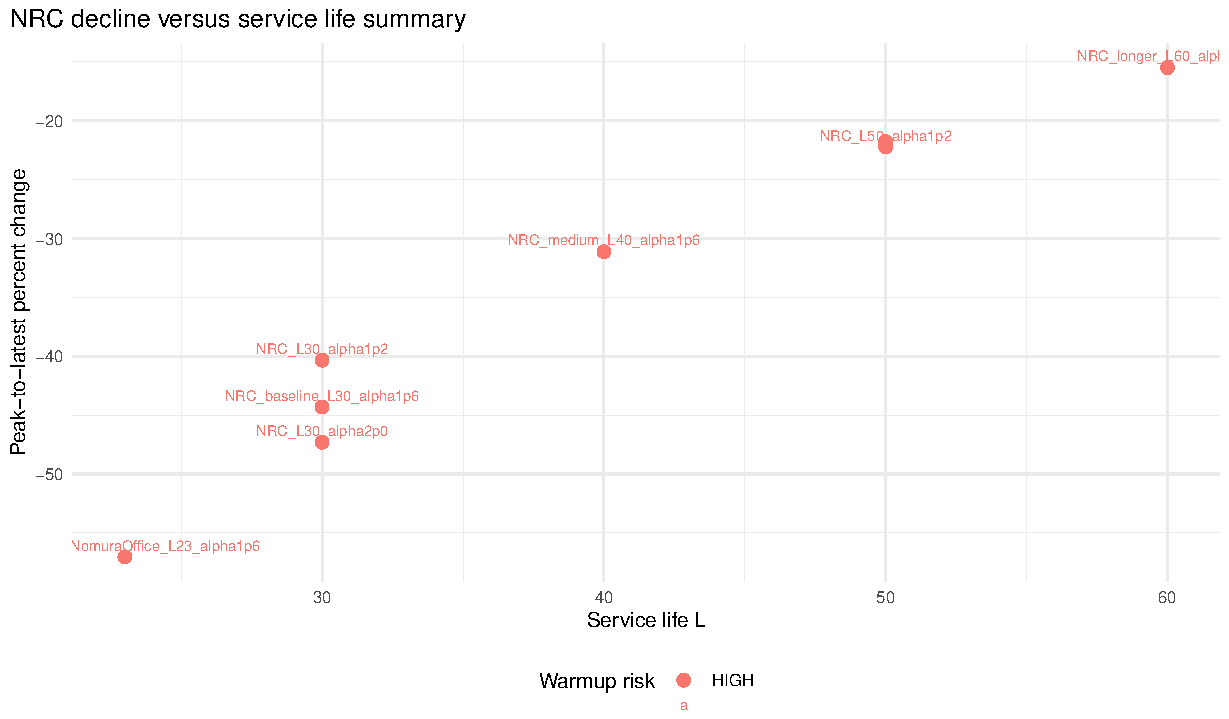
\includegraphics[width=0.92\linewidth]{../figures/D09_S_fig23_NRC_decline_vs_service_life_summary.pdf}\caption{NRC decline versus service life summary. The tradeoff is late-sample robustness versus early-sample inherited-vintage fragility.}\end{figure}\FloatBarrier
\section{What the Sensitivity Does and Does Not Authorize}
D09-S authorizes only a human-facing robustness conclusion. It does not change D06, does not rewrite D07, does not choose a new NRC service life, and does not create a model-ready transformation.
\section{Human Review Checklist}

\begin{tabular}{lllll}
\toprule
item & status & evidence & recommended\_decision & notes\\
\midrule
Nomura literature reviewed and correctly bounded & PASS & D09\_S\_literature\_source\_ledger.csv & accept & D09-S is report-only and does not authorize any sensitivity object as a model transformation.\\
Baseline D06 ME/NRC GPIM preserved & PASS & D06 md5 unchanged & accept & D09-S is report-only and does not authorize any sensitivity object as a model transformation.\\
ME service-life sensitivity visually stable & PASS & Figures 5-8 & accept & D09-S is report-only and does not authorize any sensitivity object as a model transformation.\\
NRC service-life sensitivity assessed & PASS & Figures 9-16 and decline audit & accept & D09-S is report-only and does not authorize any sensitivity object as a model transformation.\\
NRC L=30 defensibility assessed & PASS\_WITH\_REVIEW\_FLAG & D09-R and D09-S NRC ledgers & accept & D09-S is report-only and does not authorize any sensitivity object as a model transformation.\\
\addlinespace
Longer NRC service lives do not create unacceptable warmup fragility & PASS\_WITH\_REVIEW\_FLAG & Warmup audit flags longer NRC L as high review risk, not blocking & accept & D09-S is report-only and does not authorize any sensitivity object as a model transformation.\\
Stock-flow identities pass across cases & PASS & Stock-flow audit & accept & D09-S is report-only and does not authorize any sensitivity object as a model transformation.\\
Current-cost identities pass across cases & PASS & Current-cost audit & accept & D09-S is report-only and does not authorize any sensitivity object as a model transformation.\\
Capacity aggregation identities pass across cases & PASS & Capacity identity audit & accept & D09-S is report-only and does not authorize any sensitivity object as a model transformation.\\
Output-capital relations inspected across cases & PASS & Figures 19-20 & accept & D09-S is report-only and does not authorize any sensitivity object as a model transformation.\\
\addlinespace
ME/NRC composition inspected across cases & PASS & Figures 17-18 & accept & D09-S is report-only and does not authorize any sensitivity object as a model transformation.\\
No report-only sensitivity object promoted to source-of-truth & PASS & Boundary labels in ledgers and report & accept & D09-S is report-only and does not authorize any sensitivity object as a model transformation.\\
Ready to proceed to D10 transformation planning & PASS\_WITH\_NRC\_ROBUSTNESS\_FLAG & Validation checks and human flags & AUTHORIZE\_D10\_TRANSFORMATION\_PLANNING\_WITH\_NRC\_ROBUSTNESS\_FLAG & D09-S is report-only and does not authorize any sensitivity object as a model transformation.\\
\bottomrule
\end{tabular}

\section{Decision Gate}
The decision is to proceed toward D10 transformation planning with an NRC robustness flag, because the literature is bounded, the baseline is unchanged, sensitivity cases are created, identities pass, the report compiles, and there are no blocking flags.
\appendix\section{Figure Manifest}
The figure manifest is written to csv/D09\textbackslash\{\}\_S\textbackslash\{\}\_figure\textbackslash\{\}\_manifest.csv.
\section{Audit Tables}
CSV audit tables are the authoritative audit artifacts for D09-S. The human checklist is included in the main report; large ledgers remain external CSV files to avoid overfull tables.
\section{Literature Extraction Notes}
Nomura 2005 extraction located the office-building values 15.4, 22.2, and 23.0 and the SASD/Weibull/discard-survey discussion. Nomura-Futakami 2005 extraction located internal consistency, empirical verification, reproducibility, and user-testable assumption passages.
\end{document}
